\section{Interaction Language Design}
\label{sec:vg:primitives}
\subsection{Event Streams and Signals}

Reactive Vega adapts the semantics of Event-Driven Functional Reactive
Programming (E-FRP)~\cite{wan:efrp}. Low-level input events (e.g., mouse events
and keystrokes) are captured as time-varying \emph{streaming data}, rather than
event callbacks. This abstraction reduces the burden of composing and sequencing
events\,---\,operations that would require several callbacks and some external
state under an imperative paradigm. To this end, we introduce a syntax for
specifying event streams (\cref{fig:vg:eventStreams}). While prior work has
formulated regex-based symbols for event selection~\cite{kin:proton++} we
believe our approach, by drawing on CSS selectors for inspiration, will be more
familiar to designers.

\begin{figure}[h!]
  \centering
  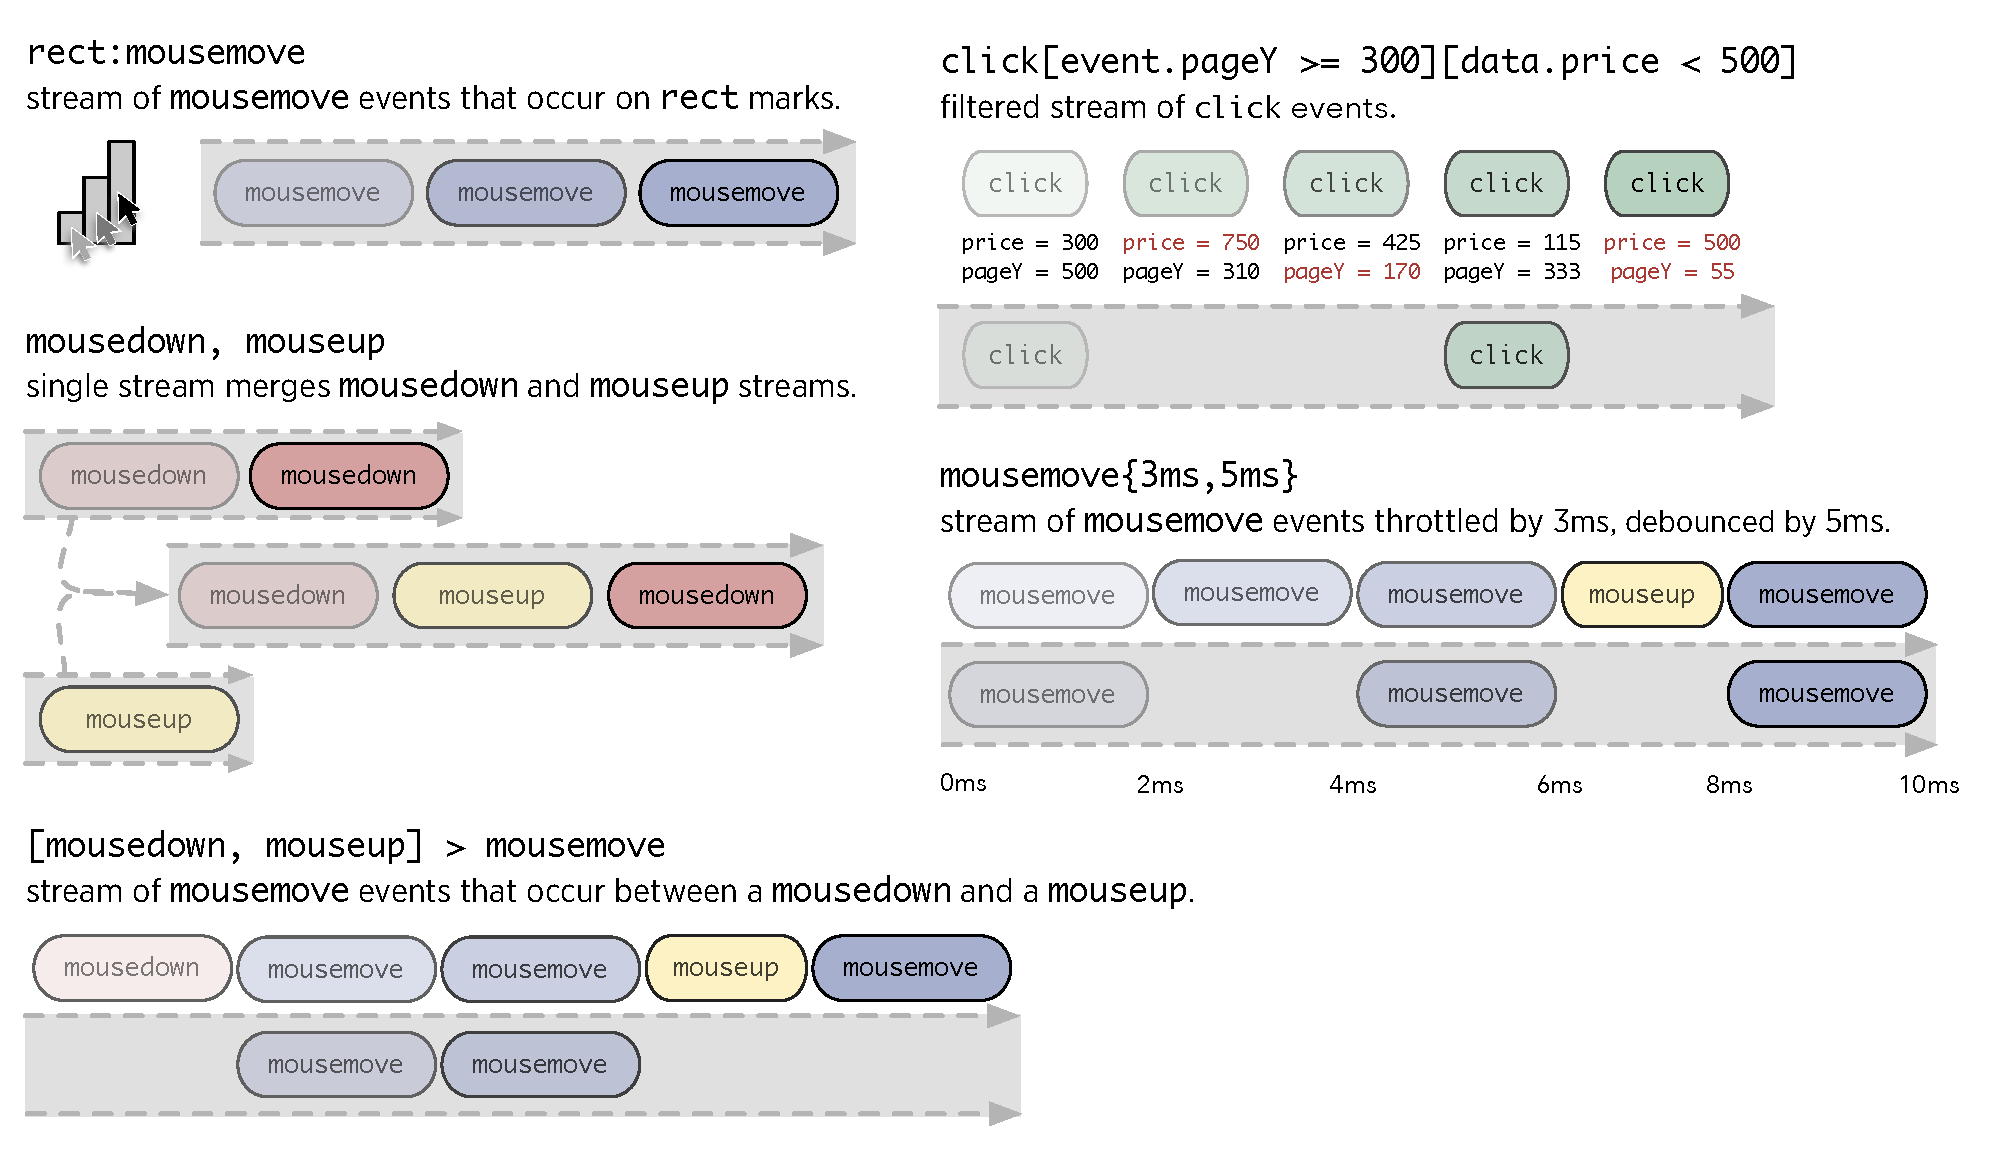
\includegraphics[width=\columnwidth]{eventStreams}
  \caption{Reactive Vega provides an event stream selector syntax, inspired by
  CSS selectors, to compose, filter, and sequence input events.}
  \label{fig:vg:eventStreams}
\end{figure}

A basic event stream selector is specified by a particular event type (e.g.,
\texttt{mousemove}), optionally prepended with the source of the
events\,---\,either a mark type (e.g., \texttt{rect:}) or mark name (e.g.,
\texttt{@cell:}). The comma operator (\texttt{,}) merges streams to produce a
single stream with interleaved events. Square brackets (\texttt{[]}) filter
events based on their properties. When followed by the right-combinator
(\texttt{>}), the brackets indicate a ``between filter,'' defining bounding
events for the stream. For instance, \texttt{[mousedown, mouseup] > mousemove}
is a single stream of \texttt{mousemove} events that occur between a
\texttt{mousedown} and \texttt{mouseup} (i.e., ``drag'' events). To throttle or
debounce an event stream, timing information can be specified between curly
braces (e.g., \texttt{\{100, 200\}} throttles a stream by 100 milliseconds and
debounces it by 200 milliseconds).  All operators are composable. For instance,
\texttt{[mousedown[event.shiftKey], window:mouseup] > window:mousemove\{100,
200\}} specifies a stream of throttled and debounced drag events that are only
triggered when the shift key is pressed.

With Reactive Vega, interaction events are a first-class data source. They can
be run through the full gamut of data transformations and can drive visual
encoding primitives. While doing so can usefully visualize a user's interaction,
for added expressivity, event streams can also be composed into reactive
expressions called \emph{signals}. By default, signals are evaluated using the
most recent event from a stream. However, by drawing from multiple event
streams, signals can define finite-state machines with each stream triggering a
transition between states.

Signals can be used to directly specify visual encoding primitives (e.g., a
mark's fill color) thereby endowing them with reactive semantics. When an event
fires, it enters appropriate streams and is propagated to corresponding signals;
signals are re-evaluated and dependent visual encodings re-rendered
automatically.

Upon definition, signals must be given unique names. These named entities are
then used to define the rest of an interaction technique. This separation
decouples input events from downstream application logic. Thus, an interaction
can be triggered by a different set of events by simply rebinding signal
declarations. As we later demonstrate, rebinding is particularly useful for
retargeting interactions or for combining otherwise conflicting interactions.

\subsection{Predicates and Scale Inversion}

Selection is a fundamental operation in interactive visualization design~
\cite{heer:generalized}. Once a selection is made, subsequent operators can be
applied to manipulate the selected items. For visual design, it can be
sufficient to make a predetermined selection (e.g., ``select all rectangles'').
With interaction design, however, selections are driven by user
input\,---\,brushing over points of interest, or adjusting a slider to filter
data.

To express interactive selections, we introduce reactive \emph{predicates}.
As shown below, predicates can be constructed either with an \emph{intensional}
definition\,---\,specifying conditions over properties of selected
members\,---\,or an \emph{extensional} one\,---\,explicitly enumerating all
members of a selection.

\begin{figure}[h!]
  \centering
  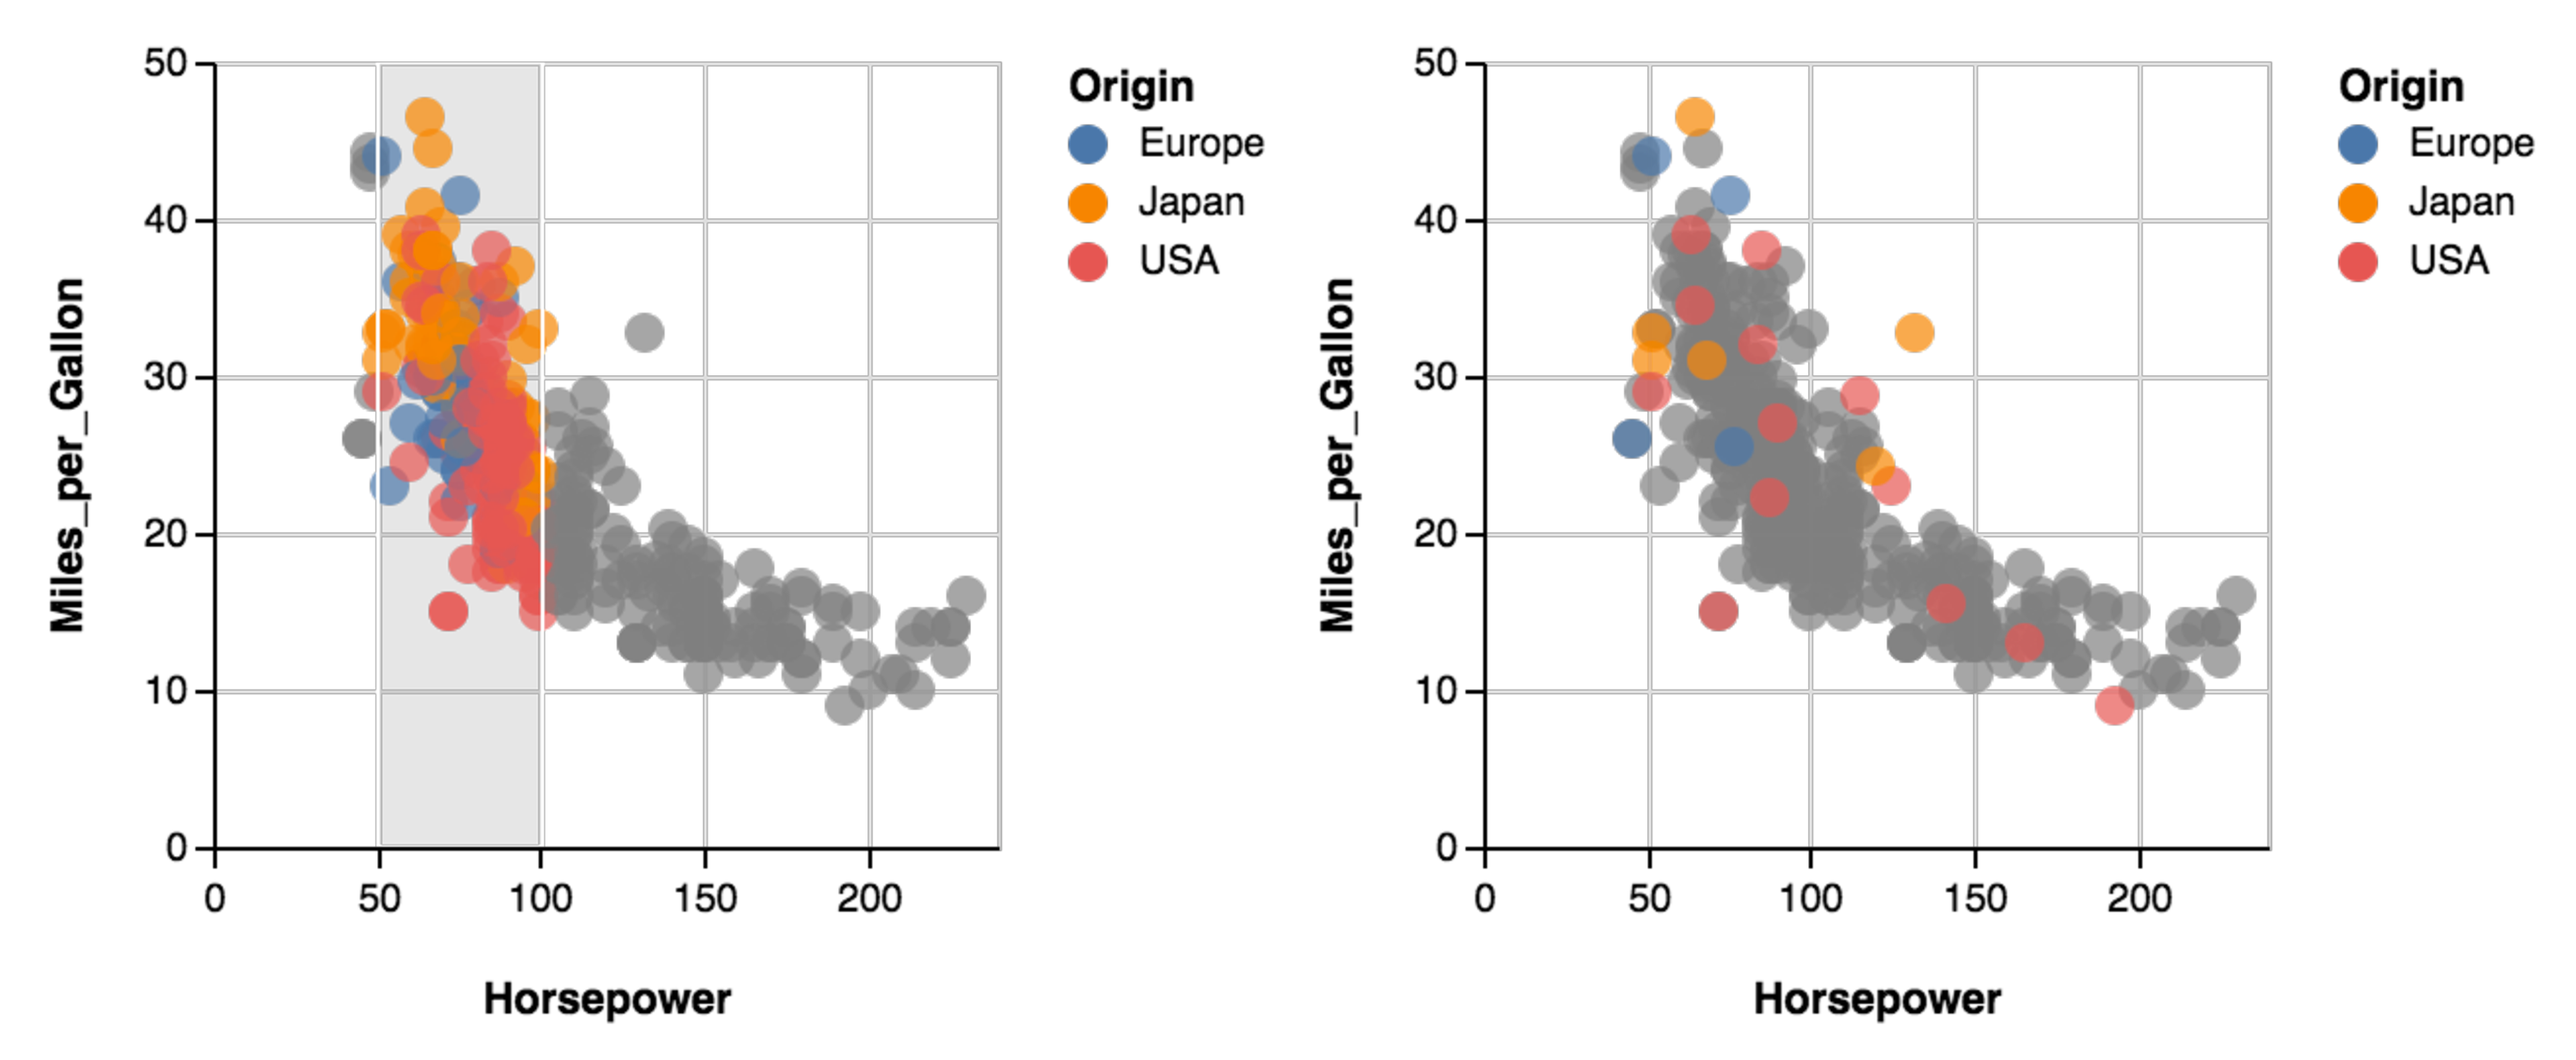
\includegraphics[width=0.9\columnwidth]{predicates}
  \caption{Points are highlighted using (left) an intensional predicate
  \texttt{50 $\leq$ Horsepower $\leq$ 100} or (right) an extensional predicate
  with members \texttt{\#56, \#110, \#79, \#95, \#40, \#120, ...}.}
  \label{fig:vg:predicates}
\end{figure}

Predicate operands are typically signals and, as signals drawn from input event
streams, predicates express interactive selections at the visual (or pixel)
level by default. However, pixel-level selection is often insufficient. A single
visualization may have multiple distinct visual spaces, or an interactive
technique may wish to coordinate multiple distinct visualizations. In such
cases, it is necessary to generalize an interactive selection into a query over
the data domain~\cite{heer:generalized}. Scale functions are a critical
component in visualization design~ \cite{wilkinson:grammar} as they transform
data values into visual values such as pixels or colors. By applying an
\emph{inverted} scale function to predicate operands, we can lift a predicate to
the data domain.

\begin{figure}[h!]
  \floatbox[{\capbeside\thisfloatsetup{capbesideposition=
  {right,center},capbesidewidth=0.3\columnwidth}}]{figure}[\FBwidth]
  {\caption{\emph{Predicates} use signal values to define interactive selections
of elements. Using \emph{scale inversions}, predicates can be generalized to
define interactive queries, and thus operate across different coordinate spaces:
overview (bottom) and detail (top).}
  \label{fig:vl:scaleInversion}}
  {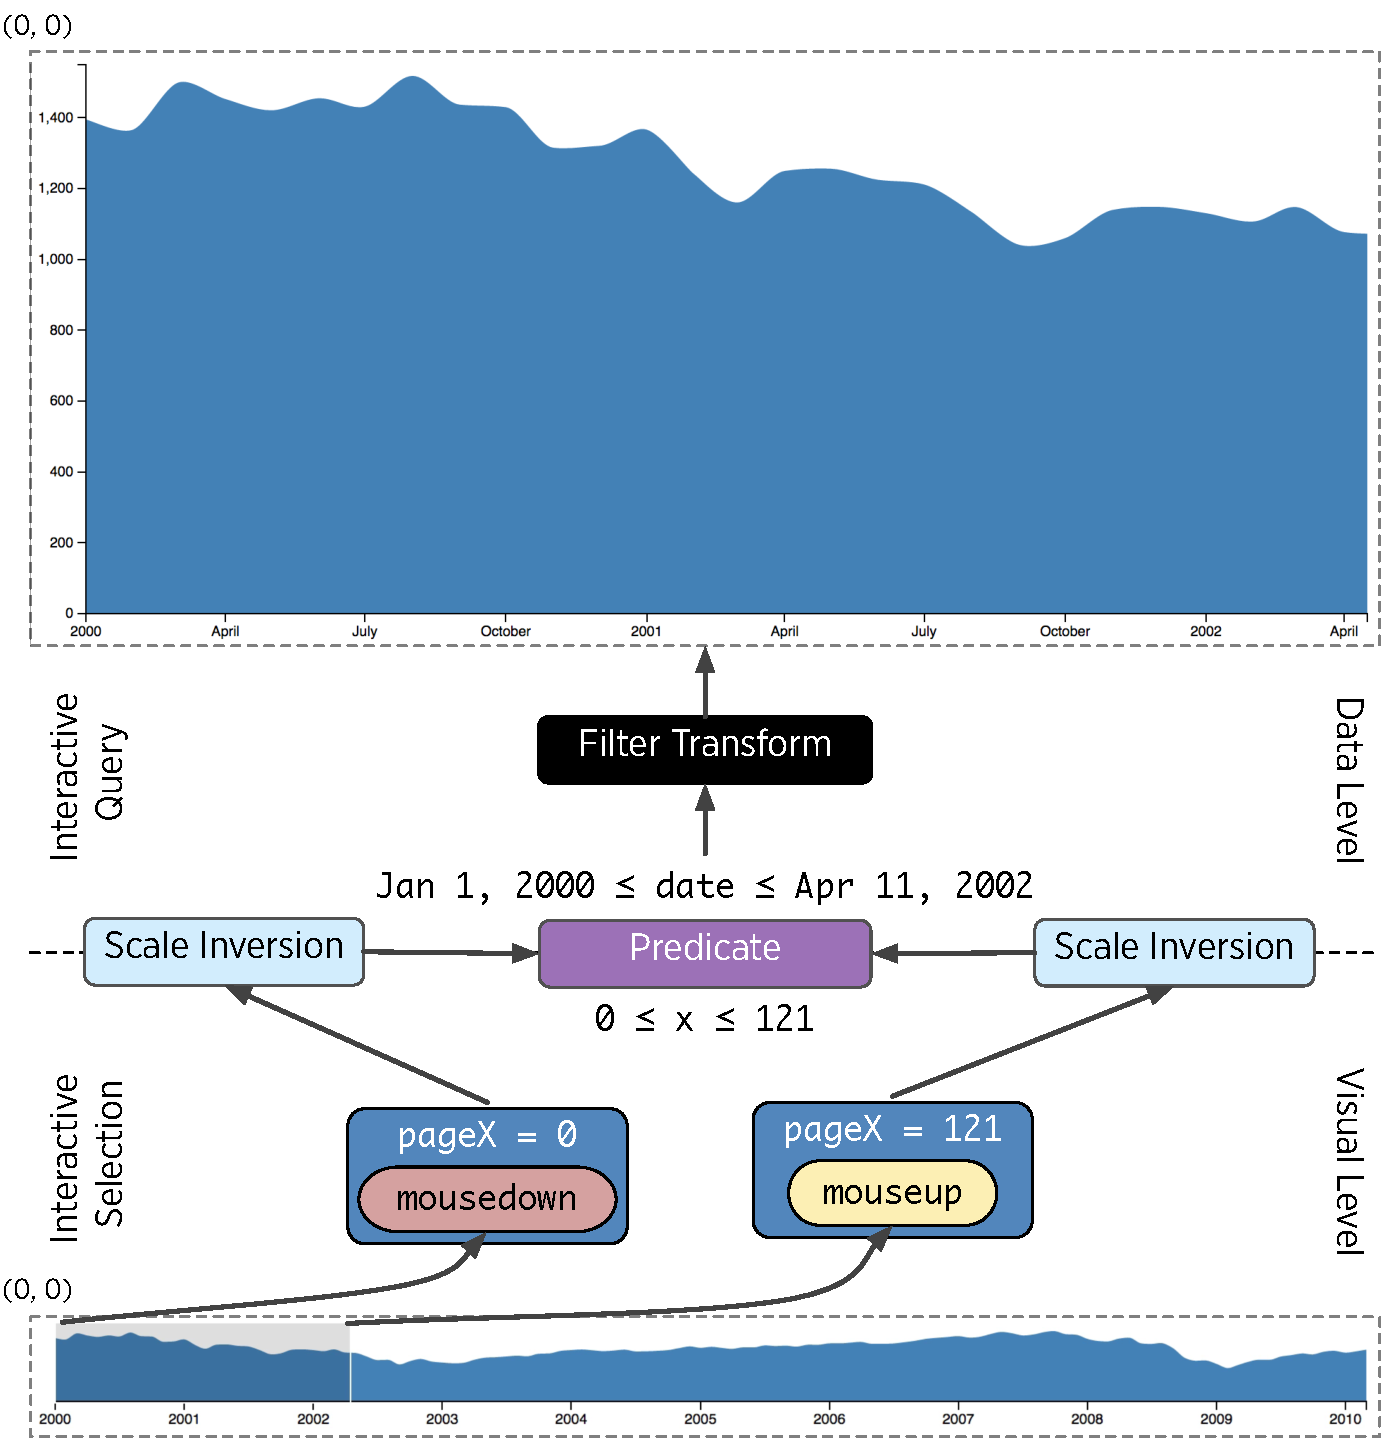
\includegraphics[width=0.7\textwidth]{scaleInversion}}
\end{figure}

\subsection{Production Rules}

Production rules are an established design pattern for visualization
specification~\cite{heer:designpatterns} that we endow with reactive semantics.
A rule defines the outcome of evaluating an \texttt{if-then-else} chain to set
property values. For example, a rule might set a mark's fill color using
scale-transformed data if predicate \texttt{A} is true, set it to yellow is
predicate \texttt{B} is true, or otherwise set the color to grey by default.

\subsection{User-Defined Functions}

During our design process, we encountered visualizations in which interactions
trigger custom data transforms. For example, sorting a co-occurrence matrix by
frequency or querying time-series data via relaxed
selections~\cite{holz:relaxed}. It is not feasible for a declarative language to
natively support all possible functions, yet custom operations must still be
expressible. Following the precedent of languages such as SQL, we provide
\emph{user-defined functions}. Such functions must be defined and registered
with the system at runtime, and can subsequently be invoked declaratively within
the specification. User-defined functions ensure that the language remains
concise and domain-specific, while ensuring extensibility to idiosyncratic
operations.

\subsection{Encapsulated Interactors}

To allow reuse of custom interaction techniques, Reactive Vega's interaction
primitives can be parameterized and encapsulated as named \emph{interactors}. An
interactor can subsequently be applied to a visualization and functions like
mixin. Its specification is merged into the host's and, to prevent conflicts,
its components are addressable only under its namespace.
\Cref{fig:vg:splomInteractor} illustrates how a brush interaction, extracted
from \cref{fig:vg:brush}, can be applied to brush \& link a scatterplot matrix.